% ----------------------------------------------------------
% Introdução
% ----------------------------------------------------------
% \section*[Introdução]{Introdução}
\cleardoublepage
\section{Introdução}
% \addcontentsline{toc}{chapter}{Introdução}

 A forma tradicional de utilizar sistemas de busca é realizar consultas por meio de palavras-chave a partir das quais o sistema responde com dados potencialmente relevantes para o usuário. Se o usuário não sabe exatamente como expressar a sua consulta, ele pode precisar refiná-la e aprimorá-la por meio de ``tentativa e erro'' até que encontre a informação que se está buscando, o que pode  tornar o processo demorado e sujeito a erros. A complementação automática de consultas é um mecanismo que pode auxiliar usuários na tarefa de busca que tem sido amplamente adotado atualmente. Essa funcionalidade consiste em, a partir de um prefixo já digitado pelo usuário, tentar ``advinhar'' a consulta final que será digitada \citep{santo2015}. Com isso, não é necessário escrever toda a consulta, o que além de poupar tempo, pode ajudar a formular uma consulta mais precisa.

\begin{figure}[htbp]
    \centering
    \begin{subfigure}[b]{0.49\textwidth}
        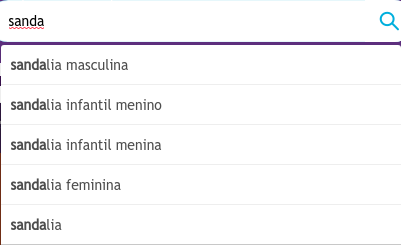
\includegraphics[width=\textwidth]{figures/autocomplete_example1.png}
        \caption{Exemplo de complementação automática de consultas comum.}
        \label{fig:common_autocomplete}
    \end{subfigure}
    \begin{subfigure}[b]{0.49\textwidth}
        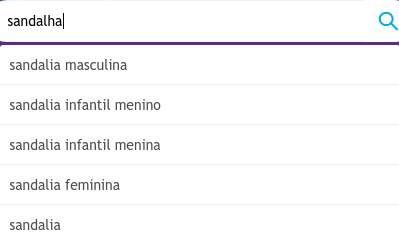
\includegraphics[width=\textwidth]{figures/autocomplete_example2.png}
        \caption{Exemplo de complementação automática de consultas tolerante a erros.}
        \label{fig:error_tolerant_autocomplete}
    \end{subfigure}
    \caption{Complementação automática de consultas em uma plataforma de \textit{e-commerce}. }
    \label{fig:query_autocompletion_example}
\end{figure}


A complementação automática de consultas pode se dar em duas formas. A primeira está representada na Figura~\ref{fig:common_autocomplete}, na qual o usuário insere o prefixo de consulta \textit{``sanda''} e o sistema automaticamente sugere cinco possíveis consultas relacionadas cujos prefixos correspondem exatamente ao que foi consultado (destacados em negrito em cada consulta). No entanto, é comum que haja erros de ortografia no conteúdo digitado. Cerca de $10\%$ a $20\%$ das consultas são digitadas erroneamente \citep{broder2009}. Para tratar tais situações é necessário que esses erros sejam considerados na busca pelas sugestões que serão retornadas. Esse problema é denominado complementação automática  tolerante a erros (CATE). Quando o usuário não sabe escrever corretamente uma palavra, é mais provável que ele consulte um prefixo com erros de digitação. A segunda forma da complementação automática, presente na Figura~\ref{fig:error_tolerant_autocomplete}, representa uma resolução para esse problema. A apesar da digitação errada do prefixo \textit{``sandalha''}, o sistema ainda assim foi capaz de mostrar sugestões cujos prefixos correspondem aproximadamente ao que foi consultado, pois sua complementação automática de consultas é tolerante a erros. Tal tolerância pode economizar os esforços do usuário de $40\%$ até $60\%$ \citep{ji2009efficient}.

Esse mecanismo pode ser visto como uma versão especializada do problema de casamento de padrão. Nesse problema, há uma janela de busca com o mesmo tamanho do padrão $p$ buscado que é movida da esquerda para a direita em um texto $t$. A cada movimento, o padrão $p$ é buscado dentro dessa janela. Esse casamento de padrão pode ser realizado de forma exata, ou aproximada. O problema de casamento exato de padrão é definido como encontrar todas as ocorrências $t_{j',j} = t_{j'}..t_{j}$ de um padrão $p = p_{1},..,p_{m}$ em um texto $t = t_{1},..,t_{n}$, sendo $m \leq n$.

Já o problema de casamento aproximado de padrão é definido como encontrar todas as sub-cadeias de caracteres $t_{j',j} = t_{j'}..t_{j}$ de um texto $t = t_{1},..,t_{n}$ cuja distância de edição para um padrão $P = p_{1},..,p_{m}$ esteja dentro de um limiar $\tau$, ou seja, $ed(t_{j',j}, P) \leq \tau$, sendo $ed(s_{1}, s_{2})$ uma função que calcula a distância de edição entre $s$ e $t$. A distância de edição entre duas cadeias de caracteres $s_{1}$ e $s_{2}$ é definida como \textit{o menor número de operações necessário para transformar $s_{1}$ em $s_{2}$}. Comumente as operações permitidas nesse contexto são a \textit{inserção}, \textit{deleção} ou \textit{substituição} de um caractere.

Essa versão aproximada do problema de casamento de padrão pode ser aplicada ao problema de CATE. Seja $p$ um prefixo de consulta digitado pelo usuário, $S=\{Q_{1}, Q_{2}, ... , Q_{n}\}$ um conjunto de $n$ cadeias de caracteres que representa todas as possíveis sugestões de consulta, e $\tau$ um limite máximo de distância de edição tolerado. O problema de CATE consiste em encontrar um subconjunto de sugestões $S'$ cujos elementos correspondem à $p$ com no máximo $\tau$ erros. Ou seja, é preciso que cada consulta presente em $S'$ possua pelo menos um prefixo que possa possa ser transformado em $p$ com no máximo $\tau$ operações de edição.

Para exemplificar, seja $\tau = 2$, $p = ``sapatho"$ e S = \textit{\{``sapatilha\ preta'', ``salaminho\ italiano'', ``sapinho\ verde''\}}. De acordo com a definição apresentada acima, o subconjunto de $S$ correspondente às consultas que serão sugeridas será \textit{S' = \{``sapatilha\ preta'', ``sapinho\ verde''\}}. No caso da consulta ``salaminho\ italiano'', seus possíveis prefixos são \textit{\{``s'', ``sa'', ``sal'', ``sala'', ... , ``salaminho italiano''\}}, e nenhum deles pode ser transformado em $p = ``sapatho"$ com no máximo $\tau = 2$ edições, portanto, ela não pode ser retornada como resposta. Por outro lado, a consulta ``sapatilha\ preta'' possui como um de seus prefixos ``sapat'', o qual pode ser transformado em $p$ com a inserção dos caracteres ``h'' e ``o'' no final (duas operações de edição). Há também a consulta ``sapinho\ verde'', com o prefixo ``sapinho'', que pode ser transformado em $p$ ao substituir a quarta e quinta letra por ``a'' e ``t'', respectivamente.

A tendência comum entre os melhores métodos propostos recentemente no estado da arte para solucionar esse problema \citep{chaudhuri2009extending,ji2009efficient,li2011efficient, xiao2013efficient,deng2016meta, zhou2016beva} é a de utilizar uma estrutura chamada  \textit{Trie} \citep{fredkintrie1960} para indexar os textos das sugestões de consulta. A \textit{Trie} é uma árvore \textit{M-ária} cujos nós são vetores de tamanho $M$ contendo em suas células caracteres que pertencem a um alfabeto $\Sigma$. O nó raiz $\epsilon$ representa uma cadeia de caracteres vazia. Cada nó em um nível $l$ representa o conjunto de todas os elementos que começam com uma sequência $p$ (que pode ser obtida ao caminhar partindo do nó $\epsilon$ até o nó em questão) de $l$ caracteres. Sendo assim, todos os prefixos em comum dentre os itens indexados compartilham dos mesmos nós. Quando o usuário faz uma consulta por um prefixo, esses métodos utilizam a \textit{Trie} para calcular todos os prefixos similares, e a partir deles sugerir as consultas.

Porém, uma vez que cada nó da árvore pode ter até $|\Sigma|$ filhos, essa estrutura tende a consumir alta quantidade de memória quando a base de consultas indexada é muito grande e não há muitos prefixos em comum entre os itens. Essa situação pode dificultar o uso desses métodos para solucionar o problema de CATE em alguns casos. O método ICAN \citep{ji2009efficient}, por exemplo, ao indexar uma base de aproximadamente $10$ milhões de itens consome $\sim9GB$ de memória. 

Além disso, o complemento automático de consultas em sistemas de busca deve ocorrer muito rapidamente, de forma quase imperceptível para o usuário. Para isso, cada complementação deve ocorrer em menos de $100ms$ \citep{ji2009efficient}, considerando inclusive a latência de rede entre a máquina do usuário e o servidor que processa as consultas.

Uma possível abordagem para diminuir o uso de memória utilizado para processar as consultas é a estratégia de busca em dois níveis. No primeiro nível, é possível realizar a busca em um índice \textit{Trie} que indexa somente uma parte inicial dos textos da base de sugestões de consulta. As folhas encontradas por essa busca podem estar associadas com um conjunto de itens, em vez de um único texto (restante da sugestão de consulta). Então, no segundo nível, cada elemento desse conjunto é analisado (um por um, de forma sequencial) para determinar quais sugestões desse conjunto de fato vão ser sugeridas. 

Costa Xavier \citep{xavier2019} realizou um trabalho preliminar que confirmou a hipótese de que é possível utilizar uma estrutura de busca em dois níveis para o problema de complementação automática de consultas tolerante a erros. Em sequência, Gama Ferreira \citep{berg2020} aprimorou significativamente a busca em dois níveis ao utilizar utilizar o mesmo algoritmo (BEVA) de busca nos dois níveis da \textit{Trie} e ao apresentar uma nova estratégia de inserção de chaves em seu índice que acelera o processamento das consultas por utilizar o sistema de cache das máquinas de maneira mais eficiente. % ideia do "level at a time" -> muito boa :)!

A abordagem em dois níveis pode proporcionar uma ótima redução do uso memória como dito anteriormente. No entanto, um dos maiores problemas com essa abordagem é o aumento do tempo de processamento necessário para sugerir consultas para um prefixo, pois a classe de complexidade computacional da busca sequencial realizada no segundo nível normalmente está acima da classe de complexidade dos algoritmos de busca que podem ser utilizados nas árvores \textit{Trie} do primeiro nível.

Neste trabalho nós estudamos alternativas para otimizar a busca em uma estrutura em dois níveis com o objetivo de computar as complementações de consulta tolerando erros com um bom desempenho aliado à redução da memória utilizada. Investigamos os impactos de uma heurística que visa aproveitar informações de erros de distância de edição provenientes do processamento da consulta no primeiro nível para acelerar o processamento no segundo nível. Também estudamos os efeitos da aplicação dessa heurística no tempo de processamento e na cobertura de resultados (medição de quantas sugestões o método deixou de encontrar e quantas sugestões encontradas na verdade não deveriam ser consideradas). 

Para implementar as ideias propostas, utilizamos o algoritmo ICPAN \citep{li2011efficient}, o qual é uma otimização do algoritmo ICAN \citep{ji2009efficient} para realizar a busca no índice \textit{Trie} no primeiro nível. Ambos utilizam uma estratégia incremental que consiste em processar um prefixo de consulta $p=c_{1}c_{2}...c_{x}$ caractere a caractere, e ``ativar'' nós da árvore \textit{Trie} a cada etapa do processamento. Para o i-ésimo caractere processado, cada nó ativo $n$ representa um prefixo cuja distância de edição $n_{d}$ entre o prefixo $p'=p[c_{1}..c_{i}]$ é menor ou igual ao limite de tolerância $\tau$ estabelecido. O ICPAN é mais eficiente que o ICAN pois utiliza um conceito de ``nós ativos pivotais'' para reduzir o conjunto de nós ativados durante toda a computação. Essa redução implica que menos itens precisarão ser verificados no segundo nível, portanto é vantajosa para a abordagem em dois níveis.

No segundo nível, verificamos que em alguns casos é possível realizar uma busca binária em vez de uma busca sequencial. Então, estudamos o quão efetiva seria uma abordagem que combina a estratégia de realizar tanto buscas sequenciais quanto binárias no segundo nível. Percebemos que quando estabelecemos a restrição de que todas as sugestões de consulta retornadas pelo nosso método estejam totalmente de acordo com a definição do problema de CATE, essa otimização só pode ser aplicada em cerca de $15\%\sim20\%$ dos casos. Consequentemente, a melhora no tempo de processamento não foi tão expressiva quanto o esperado. No entanto, nossos experimentos demonstraram que utilizando no máximo $35\%$ da memória requerida pelo ICAN e ICPAN o método em geral obteve uma média de tempo de processamento menor que a do ICAN.
\textbf{TODO: verificar novamente essas conclusões e ajeitar o que for necessário}

Além disso, é possível suavizar essa restrição, de forma que o método deixa de trazer alguns resultados e passa a trazer outros que não deveriam ser considerados, mas agora possibilitando que a otimização seja aplicada em cerca de $85\%\sim90\%$ dos casos, o que pode deixar o tempo de processamento até duas vezes mais rápido, como demonstrado em alguns dos nossos experimentos. Considerando essa suavização, podemos levantar estes questionamentos: ``Em um sistema de busca real, qual é o impacto que o nosso método com a restrição suavizada pode causar na experiência final do usuário?''; ``O quanto essa ausência ou acréscimo de algumas sugestões de consultas atrapalha a navegabilidade o usuário?''; Na Seção~\ref{sec:results} realizamos um experimento com uma base de sugestões de consultas e de prefixos consultados proveniente de um sistema real que implementa a complementação automática de consultas tolerante a erros, com o objetivo de explorar essas perguntas pertinentes.

\subsection{Problema de Pesquisa}
\label{sec:research-problem}
A principal hipótese estudada nesta dissertação é a de que é possível implementar um sistema de complementação automática em dois níveis combinando busca sequencial e busca binária no segundo nível, de forma que a eficiência do processamento aumente e que a acurácia dos resultados não seja prejudicada. As propostas apresentadas por Costa Xavier e Gama Ferreira indicam que a busca em dois níveis é uma abordagem promissora para sistemas de complementação automática. Ao iniciar esta pesquisa, tivemos a ideia de combinar busca binária com sequencial no segundo nível. Apesar de parecer uma ideia simples a princípio, sua implementação trouxe consigo desafios que são apresentados ao longo do trabalho. Nossa pesquisa teve como objetivo responder às seguintes questões de pesquisa: i) É possível adaptar sistemas de busca em dois níveis para tirarem proveito da busca binária no segundo nível? ii) Quais são as adaptações necessárias e limitações de uso da ideia? iii) Há vantagens práticas na combinação de busca binária e busca sequencial no segundo nível?


O restante desta dissertação está organizado da seguinte forma: Na Seção~\ref{sec:related_work} nós mostramos os trabalhos relacionados e os algoritmos existentes na literatura que abordam o problema de complementação automática de consultas tolerante a erros. Na Seção~\ref{sec:ref_teorico} introduzimos uma definição formal do problema e detalhamos alguns conceitos necessários para uma compreensão mais completa do trabalho. Na Seção~\ref{sec:metodo} detalhamos a implementação do método em dois níveis proposto, juntamente com a heurística de otimização do segundo nível, e os detalhes da suavização da restrição de cobertura de resultados. Na Seção~\ref{sec:results} apresentamos e analisamos os resultados dos experimentos realizados, e por fim, na Seção~\ref{sec:conclusion}, comentamos nossas conclusões do trabalho e também possíveis direções para trabalhos futuros.
